\chapter{Artificial Neural Networks}

\section{Theory}
Artificial Neural Networks (ANN) also called multilayer perceptron, can be used as a model for pattern recognition. 
In the linear models of classification is based on linear combinations of fixed nonlinear basis function $ \phi_j(x)$ on the form
\begin{equation}
y(\mathbf{x},\mathbf{w}) = f\left( \sum_{j=1}^{M}w_j \phi_j(x) \right)
\label{eq:basisF} 
\end{equation}
ANN can extend this model by allowing the basis function $ \phi_j(x)$ to depend on parameters and then to allow these parameters to be adjusted together with the coefficients $ \left\lbrace w_j \right\rbrace $, during the training phase.

The basic neural network model, which is a series of functional transformations. 
In the model the input variables is a $ M $ linear combination $ x_1,...,x_D $ on the form
\begin{equation}
a_j = \sum_{i=1}^{D} w_{ij}^{(1)}x_i+w_{j0}^{(1)}
\end{equation}
Where $ j=1,...,M $ and superscript (1) is corresponding to the parameters of the first layer of the network.
The parameters $ w_{ij}^{(1)}$ and $w_{j0}^{(1)} $ is respectively the weights and the biases. 
The quantities $ a_j $ are called activations, each of them is transformed by an activation function $ h(\cdotp) $, resulting in $ z_j = h(a_j) $.
Which correspond to the output of the basis function in \ref{eq:basisF}, that in neural network is called hidden units. Using the method of equation \ref{eq:basisF}, these quantities gets linearly combined again to give output unit activations  
\begin{equation}
a_k = \sum_{j=1}^{M} w_{kj}^{(2)}z_j+w_{k0}^{(2)}
\end{equation}
where $ k = 1,...,K $ and $ K $ is the total numbers of outputs. 
This is the second transform and therefore corresponds to the second layer of the network.
The output unit activations can be transformed using another activation function, resulting in a set of network outputs $ y_k $.
The activation function is chosen depending on the data and distribution.
In a multiple binary classification problem, each output unit activation is transformed using a logistic sigmoid function:
\begin{equation}
y_k = \sigma(a_k), \qquad \sigma(a) = \dfrac{1}{1+\mathtt{exp}(-a)}
\end{equation}
   
\begin{figure}[H]
\centering
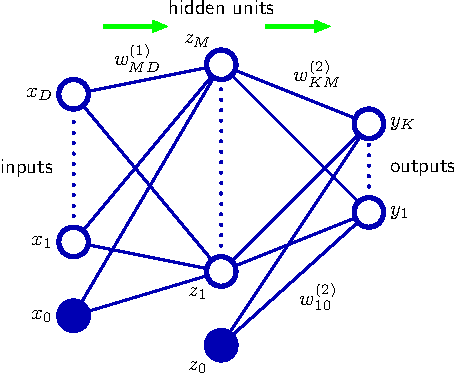
\includegraphics{Figure5_1}
\caption{Results of using ANN with 3 speakers, 30 hidden variables and 1 digit spoken}
\label{fig:ANN_fig_theory}
\end{figure}

\section{Method}



\section{Result}


\subsection{Single digit:}
\begin{figure}[H]
\centering
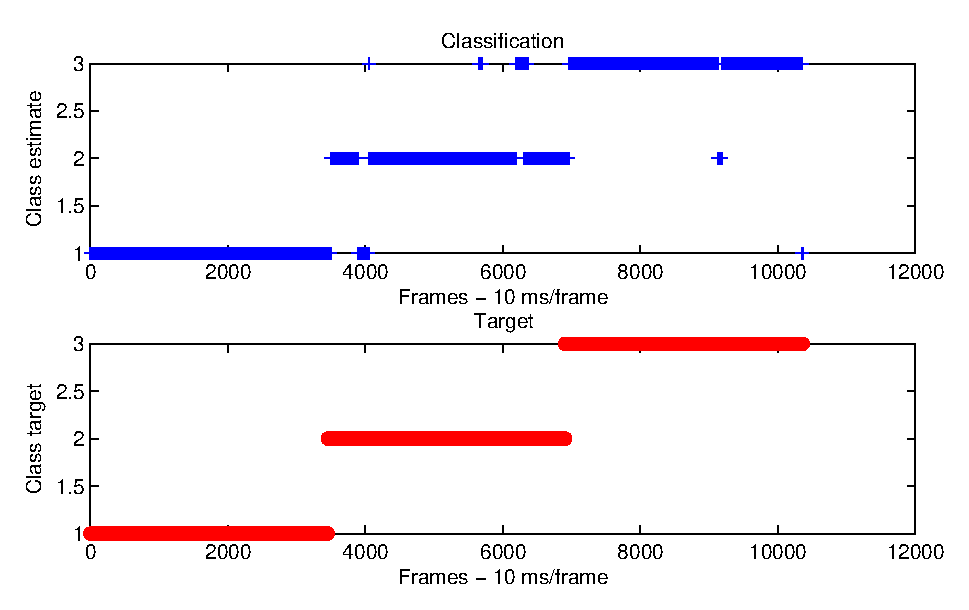
\includegraphics{ANN_1digit_8cent_3speak}
\caption{Results of using ANN with 3 speakers, 30 hidden variables and 1 digit spoken}
\label{fig:ANN_fig_1}
\end{figure}

\begin{table}[H]                                                    
\centering                                                          
\begin{tabular}{|l|c|c|c|c|}                                        
\hline                                                              
  & Speaker Jacob & Speaker Mose & Speaker Simon & Precision [\%] \\
\hline                                                              
Estimate Jacob & 3454.0 & 196.0 & 11.0 & 94.3 \\                    
\hline                                                              
Estimate Mose & 0.0 & 3077.0 & 104.0 & 96.7 \\                      
\hline                                                              
Estimate Simon & 0.0 & 181.0 & 3339.0 & 94.9 \\                     
\hline                                                              
Sensitivity [\%] & 100.0 & 89.1 & 96.7 & 95.3 \\                    
\hline                                                              
\end{tabular}                                                       
\caption{Confusion matrix - 1 digit}                                
\label{table:ANN_conf_1}                                            
\end{table}  



\subsection{Two digits:}
\begin{figure}[H]
\centering
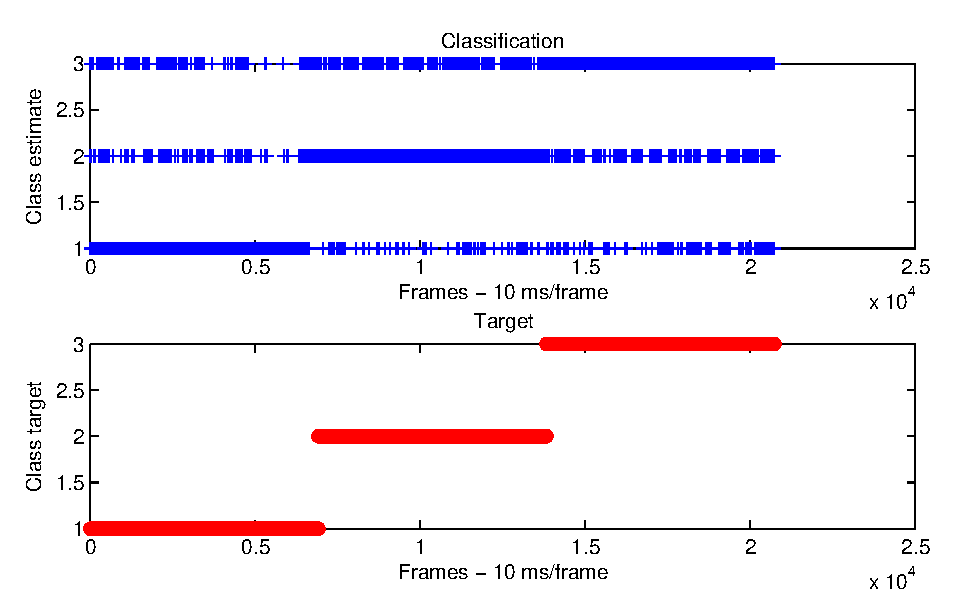
\includegraphics{ANN_2digit_8cent_3speak}
\caption{Results of using ANN with 3 speakers, 30 hidden variables and 2 digits spoken}
\label{fig:ANN_fig_2}
\end{figure}

\begin{table}[H]                                                    
\centering                                                          
\begin{tabular}{|l|c|c|c|c|}                                        
\hline                                                              
  & Speaker Jacob & Speaker Mose & Speaker Simon & Precision [\%] \\
\hline                                                              
Estimate Jacob & 6486.0 & 0.0 & 93.0 & 98.6 \\                      
\hline                                                              
Estimate Mose & 276.0 & 6485.0 & 492.0 & 89.4 \\                    
\hline                                                              
Estimate Simon & 148.0 & 425.0 & 6325.0 & 91.7 \\                   
\hline                                                              
Sensitivity [\%] & 93.9 & 93.8 & 91.5 & 93.1 \\                     
\hline                                                              
\end{tabular}                                                       
\caption{Confusion matrix - 2 digits}                               
\label{table:ANN_conf_2}                                            
\end{table}



\subsection{Ten digits:}
\begin{figure}[H]
\centering
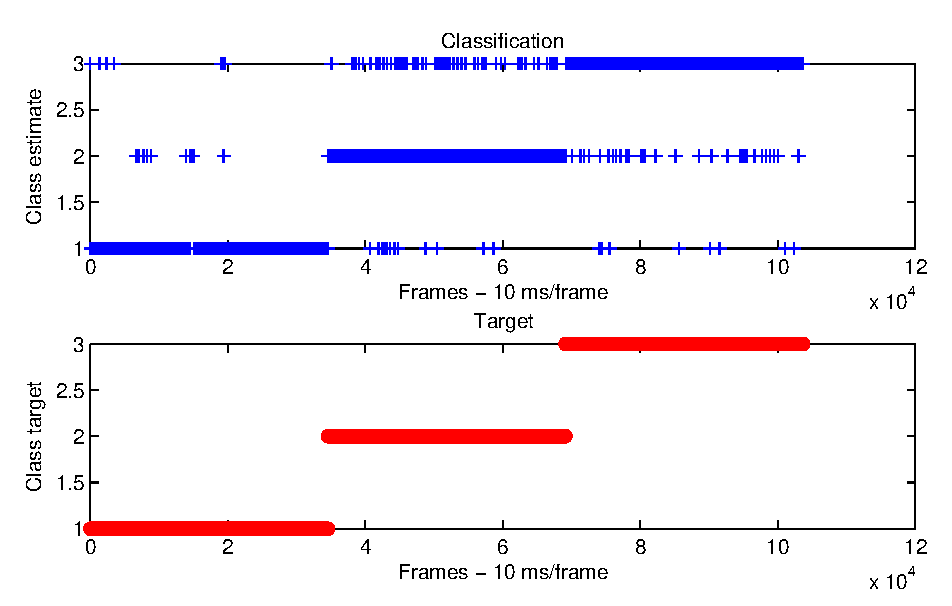
\includegraphics{ANN_10digit_8cent_3speak}
\caption{Results of using ANN with 3 speakers, 30 hidden variables and 10 digits spoken}
\label{fig:ANN_fig_10}
\end{figure}

\begin{table}[H]                                                    
\centering                                                          
\begin{tabular}{|c|c|c|c|c|}                                        
\hline                                                              
  & Speaker Jacob & Speaker Mose & Speaker Simon & Precision [\%] \\
\hline                                                              
Estimate Jacob & 32915.0 & 1186.0 & 528.0 & 95.1 \\                 
\hline                                                              
Estimate Mose & 1245.0 & 28807.0 & 3100.0 & 86.9 \\                 
\hline                                                              
Estimate Simon & 399.0 & 4566.0 & 30931.0 & 86.2 \\                 
\hline                                                              
Sensitivity [\%] & 95.2 & 83.4 & 89.5 & 89.4 \\                     
\hline                                                              
\end{tabular}                                                       
\caption{Confusion matrix - 10 digits}                              
\label{table:ANN_conf_10}                                           
\end{table}
